%% For double-blind review submission, w/o CCS and ACM Reference (max submission space)
\documentclass[sigplan,review,anonymous]{acmart}\settopmatter{printfolios=true,printccs=false,printacmref=false}
%% For double-blind review submission, w/ CCS and ACM Reference
%\documentclass[sigplan,review,anonymous]{acmart}\settopmatter{printfolios=true}
%% For single-blind review submission, w/o CCS and ACM Reference (max submission space)
%\documentclass[sigplan,review]{acmart}\settopmatter{printfolios=true,printccs=false,printacmref=false}
%% For single-blind review submission, w/ CCS and ACM Reference
%\documentclass[sigplan,review]{acmart}\settopmatter{printfolios=true}
%% For final camera-ready submission, w/ required CCS and ACM Reference
%\documentclass[sigplan]{acmart}\settopmatter{}



%\usepackage{booktabs} % For formal tables
%\documentclass{article}
%\usepackage{floatrow}
\usepackage{rotating}
\usepackage{graphicx}
\usepackage{multirow}
%\usepackage[dvipsnames]{xcolor}
\usepackage{amsfonts}
\usepackage{amsmath}
\usepackage{amssymb}
\usepackage{mathtools}
\usepackage{amssymb}
\usepackage{listings}
\usepackage{graphicx}
\usepackage{caption}
\usepackage{tabularx}
%\usepackage{amsthm}
%\usepackage[section]{placeins}
\usepackage{enumitem}
%\usepackage[a4paper, total={7in, 10.5in}]{geometry}
\usepackage[font={small}]{caption}
%\usepackage[font={bf,sf,small}]{caption}
\usepackage[linesnumbered,ruled]{algorithm2e}
\usepackage{algpseudocode}
\captionsetup{labelfont=bf,textfont=bf}
\usepackage[font={bf,sf,scriptsize}]{subfig} 
%\usepackage[demo]{graphicx}
%\setlength{\footskip}{15pt}
%\usepackage[utf8]{inputenc}
%\usepackage[english]{babel}
\newtheorem{theorem}{Theorem}[section]
\newtheorem{corollary}{Corollary}[theorem]
%\newtheorem{lemma}[theorem]{Lemma}
\newcommand\todo[1]{\textcolor{red}{#1}}
\newcommand\greg[1]{\textcolor{blue}{[Greg: #1]}}
\newcommand\mac[1]{\textcolor{red}{[Mac: #1]}}

\newcommand*\diff{\mathop{}\!\mathrm{d}}
\newcommand*\Diff[1]{\mathop{}\!\mathrm{d^#1}}

\lstset{language=C,
	keepspaces=true,
	frame=tb,
	basicstyle=\ttfamily,
	columns=fixed,
	morekeywords={enddo},
	mathescape}

\usepackage{cleveref}
\usepackage[utf8]{inputenc}
\crefname{section}{§}{§§}
\Crefname{section}{§}{§§}

\newtheorem{defn}{Definition}
\newtheorem{thm}{Theorem}
\newtheorem{clm}{Claim}
\newtheorem{crl}{Corollary}
\newtheorem{lma}{Lemma}
%\newtheorem{proof}{Proof}
%\newtheorem*{proof*}{Proof}
\newtheorem{observation}{Observation}

\newcommand{\macb}[1]{\textbf{\textsf{#1}}}

\DeclareSymbolFont{matha}{OML}{txmi}{m}{it}% txfonts
\DeclareMathSymbol{\varS}{\mathord}{matha}{83}

\acmConference[PPoPP'19]{ACM SIGPLAN Annual Symposium on Principles and Practice of Parallel Programming}{February 16--20, 2019}{Washington DC, USA}
% \acmYear{}
% \acmISBN{} 
% \acmDOI{}
\startPage{1}

%% Copyright information
%% Supplied to authors (based on authors' rights management selection;
%% see authors.acm.org) by publisher for camera-ready submission;
%% use 'none' for review submission.
\setcopyright{none}
%\setcopyright{acmcopyright}
%\setcopyright{acmlicensed}
%\setcopyright{rightsretained}
%\copyrightyear{2018}           %% If different from \acmYear

%% Some recommended packages.
\usepackage{booktabs} 
\usepackage{makecell}
\hypersetup{draft}


\begin{document}

%% Title information

\title[I/O Optimal Dimensionless Matrix Multiplication]{Breaking The Monopoly of Dimensions: I/O Optimal Dimensionless Matrix Multiplication}


\author{First1 Last1}
\authornote{with author1 note}          %% \authornote is optional;
                                        %% can be repeated if necessary
\orcid{nnnn-nnnn-nnnn-nnnn}             %% \orcid is optional
\affiliation{
  \position{Position1}
  \department{Department1}              %% \department is recommended
  \institution{Institution1}            %% \institution is required
  \streetaddress{Street1 Address1}
  \city{City1}
  \state{State1}
  \postcode{Post-Code1}
  \country{Country1}                    %% \country is recommended
}
\email{first1.last1@inst1.edu}          %% \email is recommended

%% Author with two affiliations and emails.
\author{First2 Last2}
\authornote{with author2 note}          %% \authornote is optional;
                                        %% can be repeated if necessary
\orcid{nnnn-nnnn-nnnn-nnnn}             %% \orcid is optional
\affiliation{
  \position{Position2a}
  \department{Department2a}             %% \department is recommended
  \institution{Institution2a}           %% \institution is required
  \streetaddress{Street2a Address2a}
  \city{City2a}
  \state{State2a}
  \postcode{Post-Code2a}
  \country{Country2a}                   %% \country is recommended
}
\email{first2.last2@inst2a.com}         %% \email is recommended
\affiliation{
  \position{Position2b}
  \department{Department2b}             %% \department is recommended
  \institution{Institution2b}           %% \institution is required
  \streetaddress{Street3b Address2b}
  \city{City2b}
  \state{State2b}
  \postcode{Post-Code2b}
  \country{Country2b}                   %% \country is recommended
}
\email{first2.last2@inst2b.org}         %% \email is recommended



\begin{abstract}
%
\mac{I did not touch the abstract yet, better to leave it for the very end.}
%
In this paper we address an allegedly well-known problem of distributed Matrix
Matrix Multiplication and show new optimizations both from theoretical and
implementation sides. We establish a new framework for assessing analytical
data movement lower bounds, together with deriving optimal sequential and
parallel scheduling. Our "bottom-up" parallelization technique, opposed to
state of the art "top-down" approaches is naturally agnostic to problem
dimensions and is provably optimal in all scenarios, resulting in up to
$\sqrt{3}$ times reduction in communication volume. With our fine-tuned data
layout transformations, we are able to achieve X \% peak FLOP/s running on up
to Y nodes on the Piz Daint supercomputer, beating currently fastest-known
algorithms by a factor of Z, using provably I/O optimal, robust schedule and
employing RDMA mechanisms for communication-computation overlap.
%
%Based on an existing pebble game abstraction, we come to fundamental
%observations about parallel scheduling and data reuse, deriving new tiling
%scheme for Matrix-Matrix Multiplication, achieving a tight bound of
%$\frac{2mnk}{\sqrt{S}}$ I/O operations. We show the new NP-hardness proof for
%I/O optimal scheduling.
%
\end{abstract}


\keywords{I/O complexity, scheduling, pebble games}

%% \maketitle
%% Note: \maketitle command must come after title commands, author
%% commands, abstract environment, Computing Classification System
%% environment and commands, and keywords command.
\maketitle

\section{Introduction}
\label{sec:intro}

%To-G: One paragraph must serve *one* specific goal that one must be able to
%state in one short (~10 words at most) sentence. The previous intro was one
%large bulk of text - not good. I split into paragraphs below. Double check if
%you understand *exactly* why the division into paragraphs is like this.

Matrix multiplication (MM) is one of the most fundamental building blocks in
scientific computing. It is widely used not only in virtually all linear
algebra algorithms (Cholesky and LU decomposition~\cite{meyer2000matrix},
eigenvalue factorization~\cite{chatelin2012eigenvalues}, triangular
solvers~\cite{linearAlgebraLAPACK}), but also in numerous graph algorithms such
as Breadth-First Search (BFS)~\cite{cormen2009introduction} or Triangle
Counting~\cite{azad2015parallel} through efforts such as
GraphBLAS~\cite{kepner2016mathematical}.  Other use cases include spectral
clustering~\cite{ng2002spectral} or machine
learning~\cite{abadi2016tensorflow}.  Thus, improving the performance or
programmability of MM routines is of great significance for many domains.

%
The evolution of MM algorithms is marked by a series of important optimizations
and novel approaches, including Strassen-like routines~\cite{Strassen}, 
parallelization~\cite{parallelMMM},
and tiling~\cite{tiling}.
%
While the largest focus has been traditionally placed on accelerating the
multiplication of square matrices, more emphasis has recently been placed on
non-square matrices as well. Such matrices are commonly used in a number of
relevant areas and problems, for example in machine learning
\cite{rectangularML} or computational chemistry \cite{rectangularChemistry}.
%
Unlike square matrices, the dimensions of non-square matrices can vary
significantly. Developing MM algorithms that achieve high performance for
arbitrary dimensions is hard~\cite{sth}.
%
This issue is tackled by the recent work by Demmel et al.~\cite{CARMA}, who
introduced CARMA, an algorithm that achieves asymptotic lower bounds for all 
configurations of dimensions and intra-node memory sizes.

Unfortunately, we first observe that the recursive structure of CARMA is
unsuitable for scenarios when the number of processes is not the power of two,
a common case in practice~\cite{sth} \mac{This should be really
supported with one sentence stating and citing example applications, 
*trust me here*}. Furthermore, we emphasize that asymptotic complexity is an
insufficient measure of speedup in practical applications as constants do play
crucial role in applicability of algorithms. For example, the
Coppersmith--Winograd algorithm~\cite{coppersmith} achieves computational
complexity of $\mathcal{O}(N^{2.376})$, but its constant terms are prohibitively big and
make it slower in practice than the classical $\mathcal{O}(N^{3})$ algorithms. 
We later (\cref{sec:evaluation}) show that CARMA constant factors are also 
suboptimal in terms of communication volume.

In this work, we present a new approach to multiplying matrices that alleviates
the above issues. Our key idea is to ``invert'' the traditional ``top-down''
approach for multiplying matrices, shared by all the mentioned state-of-the-art
algorithms, that fix the domain partitioning in some predefined fashion
(2D~\cite{d1}, 2.5D~\cite{d2}, 3D~\cite{d3}, or
recursive~\cite{d4}).
%
Instead, we propose a ``bottom-up'' approach that (1) starts with deriving a
provably optimal sequential data movement schedule, (2) uses it to generate a certain
number of parallelization strategies of a given MM product, and finally (3)
uses these strategies to provide an \emph{I/O optimal} parallel schedule.
%
Our schedule is based on the ``S--partitioning'' concept from the Hong and 
Kung's 
red--blue
pebble game~\cite{redblue} to derive the best (i.e., optimal) partitioning
routine that minimizes data movement for a given MM product in a parallel
setting.
%
We illustrate an intuitive comparison of our bottom-up approach versus the
classic top-down schemes in Figure~\ref{fig:topdown-vs-bottomup}.

\begin{figure}[!tbp]
\centering
%
\subfloat[3D domain
decomposition]{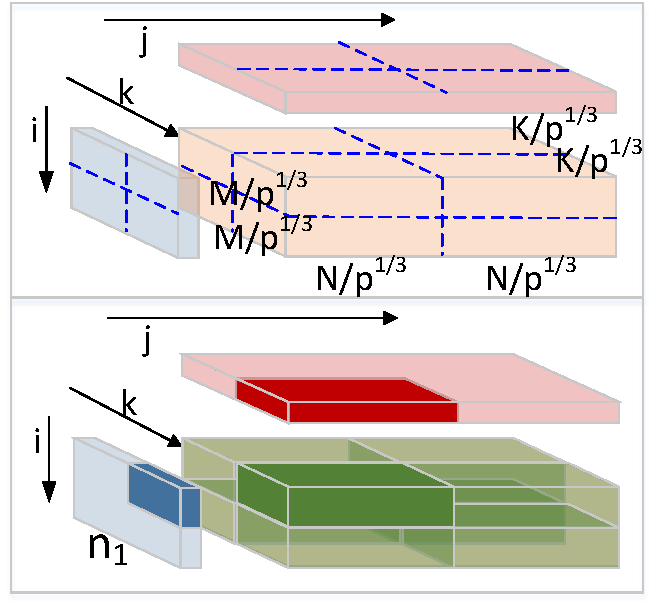
\includegraphics[width=0.22\textwidth]{figures/mmm_shape_3d}\label{fig:f1}}
%
\hfill
%
\subfloat[Domain 
decomposition based on S--partitions]{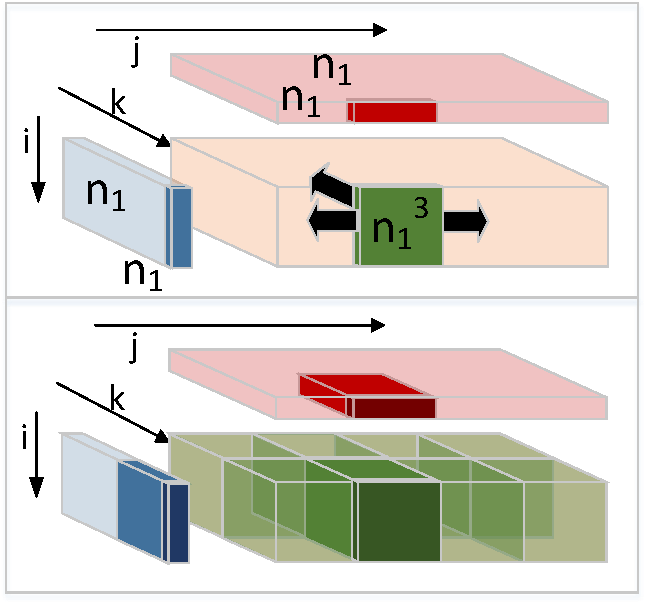
\includegraphics[width=0.22\textwidth]{figures/mmm_shape_spart}\label{fig:f2}}
%
\caption{Difference between "top-down" approach, where a global domain is
uniformly partitioned into $p$ subdomains (a), and "bottom-up", where locally
optimum subdomain fills the global domain (b). In this example, (b) has 25\%
smaller input size per process. Exact comparison is presented in Table 
\ref{tab:summary}. \mac{This figure might be OK for a technical report,
but it's too complex for the submission. Also, it should be black-white.
I also have an idea of making it in 2D. Let's discuss it when you're here.}}
%
\label{fig:topdown-vs-bottomup}
\end{figure}

Our algorithm performs from $\frac{5}{3 \sqrt[3]{4}}$ to $\sqrt{3}$ less
communication than CARMA for any dimension sizes and other parameters, and up
to $\max\{N,M,K\}$ times less than algorithms that target square matrices ($M,
N, K$ are matrix dimensions), like Cannon's~\cite{generalCannon} or 3D
SUMMA~\cite{summa}. The comparison of communication cost is presented in
Table~\ref{tab:summary}. 
%
We further motivate our work in Figure~\ref{fig:motivation-page-1} that
shows the advantages of our algorithm over the state of the art.  We
obtain up to ?? speedup (?? on average) in the total runtime of the MM scheme.

Unlike CARMA that is based on the recursive data layout, our implementation
enables transparent integration with the ScaLAPACK format~\cite{cite} and
delivers near-optimal computation throughput.
%
Next, as we later illustrate (\cref{sec:x}), the schedule that we obtain
naturally expresses computation-communication overlap, which can be naturally
used for even higher speedups using Remote Direct Memory Access (RDMA)
mechanisms.
%
Finally, our provably I/O optimal approach is easily generalizable to other
linear algebra kernels. 

We provide the following contributions:
\mac{The contributions should reflect more or less the intro story.
Now they're really vague. Will try to fix it later.}

\begin{itemize}[leftmargin=1em]
%
\item Extending classical analysis of I/O complexity, we provide 
constant terms for data movement lower bound and present a schedule 
achieving it (Section \ref{sec:datareuse}),
%
\item we confront the parallel efficiency metric of our schedule with 
existing state-of-the art 2D and 3D matrix multiplication variants 
(Section \ref{sec:datareuse}),
%
\item we present various data layout optimizations, which reduce memory 
footprint for communication buffers and guarantees minimal reshuffling 
of input data, providing better compatibility with ScaLAPACK format 
than CARMA (Section \label{sec:implementation}),
%
\item we detach the communication granularity from computation, 
yielding flexible computation-communication overlap leveraging RDMA 
mechanism (Section \label{sec:implementation}),
%
\item we perform extensive evaluation on Piz Daint \greg{and others?} 
machine of all possible combinations of problem dimensions, memory size 
and number of processes, showing the speedup of up to ?? (?? on average), 
compared to the current state-of-the-art implementations
(Section \label{sec:evaluation}).
%
\end{itemize}

%	It is a well known fact that the main emphasis on performance analysis 
%	shifted from maximizing FLOP/s to minimizing data movement. Even though I/O 
%	optimal schemes were being designed since the first register problems 
%	occurred (\cite{pebblegameregister}, \cite{registerpebblecolor}, 
%	\cite{completeRegisterProblems}, \cite{redblue}, \cite{externalMem}), 
%	contemporary throughput-oriented architectures, like Xeon Phi 
%	\cite{XeonPhi} and GPUs 
%	\cite{gpumodel} leveraged the problem to higher importance than ever 
%	(\cite{redbluewhite}, \cite{elangoSymbolic}, \cite{energyScheduling}, 
%	\cite{communicationOptMMM}). Yet, 
%	data movement minimization, due to its 
%	combinatorial nature, is far more complicated than simple FLOP/s 
%	optimization.
%	
%	As a starting point we revisit a method proposed by Hong and Kung nearly 40 
%	years 
%	ago \cite{redblue}. Their red-blue pebble game abstraction is 
%	a simple, yet elegant and powerful tool for analyzing the I/O complexity of 
%	computations expressed in the Computation Directed Acyclic Graph (CDAG) 
%	format. The key result is a method of  deriving the I/O lower bound based 
%	on a so-called \textit{S-partition} of the input CDAG.
%	
%	In this work we show the new NP-hardness result of the
%	S-partition problem. We also discuss the origin of the problem 
%	intractability and summarize cases where either polynomial time or PTAS 
%	algorithm exists. For those cases, the polynomial time algorithm is 
%	presented. However, we note that for many practical scenarios, the constant 
%	$k$ in the exponent of time complexity $\mathcal{O}(n^k)$ may still be 
%	prohibitive. To tackle 
%	this obstacle, we derive a new ILP-based branch-and-bound algorithm 
%	inspired by a 
%	work of Elango et al. (\cite{redbluewhite}) that can scale to graphs with 
%	up to (to be evaluated) vertices. 
%	
%	There are two major challenges with the S-partition. First one is present 
%	in 
%	all methods that maximizes computational intensity (the geometric 
%	interpretation is surface-to-volume ratio minimization). The problem is 
%	that those methods do not explicitly specify the data reuse. This leads to 
%	suboptimal subset shapes, which we prove on the Matrix Matrix 
%	Multiplication example.  The other challenge with S-partition lower 
%	bound is that it does not 
%	provide any tightness guarantees. We present a method 
%	to assess both the tightness and scheduling feasibility derived 
%	directly from the S-partition.  We compare our algorithm with both 
%	well-known 
%	results for Matrix-Matrix Multiplication, FFT and stencil computations, as 
%	well as random uniform and Kronecker graphs.
%	
%	This paper is organized as follows:
%	
%	(TBD)

%\begin{table*}
%	\begin{tabular*}{\textwidth}{c c c c c c}
%		\hline
%		& 2D\cite{summa} & 2.5D\cite{25d} & 3D \cite{summa3d} & 
%		CARMA\cite{CARMA} & S-partition[here]\\
%		\hline
%		\hline
%		\begin{tabular}{c}
%			proc decomp. \\
%			$[p_m \times p_n \times p_k]$
%		\end{tabular}
%		& $[p^{\frac{1}{2}} \times p^{\frac{1}{2}} \times 1]$
%		&
%		\begin{tabular}{c}
%		$[(p/c)^{\frac{1}{2}} \times (p/c)^{\frac{1}{2}} \times c]$, \\
%		$c = \frac{MK + NK}{pS}$
%		\end{tabular} 
%
%		& $[p^{\frac{1}{3}} \times p^{\frac{1}{3}} \times p^{\frac{1}{3}}]$
%		& \begin{tabular}{c}
%			$[{2^{a_1}} \times {2^{a_2}} \times 
%			{2^{a_3}}]$,\\
%			 $a_1 + 
%			a_2 + a_3 = \log_2(p)$
%		\end{tabular}
%		& 
%		\begin{tabular}{c}
%			%$[\frac{M}{T_1} \times \frac{N}{T_1} \times \frac{K}{T_1}]$ or 
%			$[\frac{M}{T_1} \times \frac{N}{T_1} \times \frac{K}{T_2}]$,\\
%			 $T_1, T_2$:  Section \ref{sec:partitionShape}
%			%  $= \frac{MNK}{p}, T_2 \approx \sqrt{S}, T_3 = \frac{MNK}{T_2^2}$
%			\end{tabular}\\
%		\hline
%		local domain size 
%		&
%			 $\Big[\frac{M}{p^{\frac{1}{2}}} \times 
%			\frac{N}{p^{\frac{1}{2}}} \times K\Big]$
%		&
%			$\Big[\frac{M}{(p/c)^{\frac{1}{2}}} \times 
%			\frac{N}{(p/c)^{\frac{1}{2}}} \times \frac{K}{c}\Big]$
%		& 
%			$\Big[\frac{M}{p^{\frac{1}{3}}} \times \frac{N}{p^{\frac{1}{3}}} 
%			\times 
%			\frac{K}{p^{\frac{1}{3}}}\Big]$
%		&
%			$[\frac{M}{2^{a_1}} \times \frac{N}{2^{a_1}} \times 
%			\frac{K}{2^{a_1}}]$
%		& 
%			$[{T_1} \times {T_1} \times {T_2}]$
%       \\
%		\hline
%	\end{tabular*}
%\end{table*}

\begin{table*}
%
\setlength{\tabcolsep}{4pt}
\renewcommand{\arraystretch}{2}
\centering
%\footnotesize
\scriptsize
\sf
%
\begin{tabular}{lllll}
%
\toprule
%
 & \textbf{2D~\cite{summa}} & \textbf{2.5D \& 3D~\cite{25d}} & \textbf{CARMA~\cite{CARMA}} & \textbf{Our work~[Section \ref{sec:partitionShape}]} \\
%
\midrule
%
\makecell[l]{\textbf{process}\\
\textbf{decomposition} \\
$\left[p_m \times p_n \times p_k\right]$}
&
$\left[\sqrt{p} \times \sqrt{p} \times 1\right]$
&
\makecell[l]{$\left[\sqrt{p/c} \times \sqrt{p/c} \times c\right]$,\\
$c = \frac{pS}{MK + NK}$}
& 
\makecell[l]{$\left[{2^{a_1}} \times {2^{a_2}} \times {2^{a_3}}\right]$,\\
$a_1 + a_2 + a_3 = \log_2(p)$}
& 
\makecell[l]{$\left[\frac{M}{\sqrt{S}} \times \frac{N}{\sqrt{S}} \times \frac{K}{d}\right]$,\\
$d = \frac{MNK}{pS}$}
%
\vspace{1.0em}
%
\\
%
%\midrule
%
\textbf{domain size}
&
$\left[\frac{M}{\sqrt{p}} \times \frac{N}{\sqrt{p}} \times K\right]$ 
&
$\left[\frac{M}{\sqrt{p/c}} \times \frac{N}{\sqrt{p/c}} \times \frac{K}{c}\right]$
&
$\left[\frac{M}{2^{a_1}} \times \frac{N}{2^{a_1}} \times \frac{K}{2^{a_1}}\right]$
& 
$\left[{\sqrt{S}} \times {\sqrt{S}} \times {d}\right]$
%
\vspace{0.5em}
%
\\
%
\midrule
%
\makecell[l]{\textbf{communication}\\
\textbf{volume}}
&
$\frac{1}{\sqrt{p}} \left(MK + NK\right)\left(1 - \frac{1}{\sqrt{p}}\right)$
&
$\frac{1}{p \sqrt{S}} \left(MK + NK\right)\left(\sqrt{MK + NK} - \sqrt{S}\right)$
&
\makecell[l]{$2a_4 \cdot \frac{MNK}{p\sqrt{S}} + a_5 \cdot \left(\frac{MNK}{P}\right)^{2/3} - \frac{MK + NK}{p}$, \\
$\sqrt{3}\le a_4 \le \sqrt{5}$,\\
$\frac{1}{2^{2/3}} \le a_5 \le 2^{1/3}$}
& 
$S + 2 \cdot \frac{MNK}{p\sqrt{S}} - \frac{MK + NK}{p}$
%
\vspace{0.5em}
%
\\
%
\midrule
%
\makecell[l]{\textbf{``the easiest case'':}\\
$M = N = K$,\\
$S = 2\frac{N^2}{p}, p=2^{3n}$}
&
$2N^2 \left(\frac{1}{\sqrt{p}} - \frac{1}{p} \right)$
&
$2N^2 \left(\frac{1}{\sqrt{p}} - \frac{1}{p} \right)$
&
$2N^2 \left(\sqrt{\frac{3}{2p}} + \frac{1}{2p^{2/3}} - \frac{1}{p} \right)$
& 
$2N^2 \left(\frac{1}{\sqrt{2p}} \right)$
%
\vspace{1.0em}
%
\\
%
%\midrule
%
\makecell[l]{\textbf{``the hardest case'':}\\
$M = N = \sqrt{p}$,\\
$K = \frac{p^{3/2}}{4}$,\\
$S = 2\frac{NK}{p^{2/3}}, p=2^{3n + 1}$}
&
$\frac{p^{3/2}}{2}\left(1 - \frac{1}{\sqrt{p}}\right)$
&
$\frac{p^{3/2}}{2}\left(\frac{1}{p^{1/6}} - \frac{1}{\sqrt{p}}\right) + p^{1/3}$
&
$\frac{3p}{4}$
& 
$\frac{3-2^{1/3}}{2^{4/3}}p \approx 0.69 p$
%
\\
%
\bottomrule
%
\end{tabular}
%
\caption{Summary of analysis of 2D, 3D, CARMA ans S-partition parallelization 
schemes. "Easiest case" is where the matrices are square and there is no extra 
memory for redundant copies of input data. The "hardest case" is where $K >> M 
= N$ and there is space for extra $p^{1/3}$ copies. For simplicity, we assume 
that parameters are chosen such that all divisions have integer results.}
%
\label{tab:summary}
\end{table*}


\section{Background and reuse-based lemma}
\label{sec:background}

This section discusses necessary concepts of pebble games in the context of I/O 
optimality. We modify Hong and Kung's lemma (inequality 
\ref{eq:redbluebound}) to prove the tighter lower bound (inequality 
\ref{eq:reusebound}), which explicitly expresses data reuse. In the context 
of matrix multiplication, the original one takes an upper bound of the data 
reuse and corresponds to case b) in Figure \ref{fig:mmmreuse}. Our result 
maximizes the achievable reuse, showed in case c) in Figure \ref{fig:mmmreuse}.
Readers not interested in deriving Lemma \ref{eq:reusebound} may proceed 
directly to Section \ref{sec:datareuse}.
The most important
symbols are gathered in Table~\ref{tab:symbols}.
%
\mac{This whole paragraph is extremely confusing, let's chat.}

\begin{table}[h!]
	\centering
	\footnotesize
	%\scriptsize
	%\ssmall
	\sf
	\begin{tabular}{@{}l|ll@{}}
		\toprule
		\multirow{7}{*}{\begin{turn}{90}\textbf{RB pebble game}\end{turn}}
		& $G$&A directed acyclic graph $G=(V,A)$\\
		%& $n,m$&Numbers of vertices and edges in $G$; $|V| = n, |E| = m$.\\
		& $S$ & Number of red pebbles (size of the fast memory)\\
		& $B = \infty$ & Number of blue pebbles (size of the slow memory)\\
		& $Dom(V_i), Min(V_i)$ & Dominator and minimum sets of subset $V_i$\\
		& $H(S)$ & Minimum cardinality valid S-partition \\
		& $R(S)$ & Maximum reuse volume between subsets \\
		& $Q$ & Minimal number of I/O operations of any valid \\ 
		& & execution of $G$ \\
		\midrule
		\multirow{3}{*}{\begin{turn}{90}\textbf{geometric}\end{turn}}           
		& $\mathcal{S}$ & Surface of a subcomputation (size of the 
		inputs \\
		& &  and outputs)\\
		& $\mathcal{V}$ & Volume of a subcomputation (number of \\
		& & 
		operations) bounded by $\mathcal{S}$\\
		& $\rho = \mathcal{V}/\mathcal{S}$ & Computational 
		intensity \\
		\midrule
		
		%\multirow{1}{*}{\begin{turn}{90}\textbf{.}\end{turn}}
		%                    & $S$ & The number of .\\
		\bottomrule
	\end{tabular}
	%\vspace{-0.5em}
	\caption{The most important symbols used in the paper.}
	\label{tab:symbols}
	\vspace{-0.5em}
\end{table}

\subsection{Modeling Program Execution}

Modeling computation as a graph pebbling problem dates back to
70s~\cite{completeRegisterProblems, pebblegameregister, registerpebblecolor}.
More specifically, we represent a computation $C$ with a directed acyclic graph
(DAG) $G=(V,E)$, where $V$ is a set of vertices and represents each
elementary operation in $C$, and the set of edges $E$ represents the data
dependencies between operations $V$. The \textit{pebbling} of a computation DAG
is a series of allowed moves, according to pre-defined rules (e.g., placing, 
removing or
moving a pebble from one vertex to another) such that certain criteria are met
- usually that all the vertices without any children (output vertices) contain
a certain pebble.

\subsection{Modeling I/O Complexity}
\noindent
\macb{Pebble Games}
%
We use \emph{pebble games} to model I/O computations in a two-level memory
structure (e.g., with caches and DRAM or DRAM and external storage).  We focus
on \emph{the red-blue pebble game} by Hong and Kung~\cite{redblue}.
%
In this model, one first places a set of $k$ blue pebbles on $k$ input DAG
vertices (this corresponds to initializing the slow memory with the input data
of size $k$).  One later applies several \emph{rules} until the final
configuration of pebbles is obtained (corresponding to producing the desired
output). Applying these rules corresponds to the actual computation in the I/O
setting with a two-level memory hierarchy.  The rules are as follows. First,
one can place a red pebble on any vertex with a blue pebble (this corresponds
to copying data from the slow to the fast memory).  Second, one can place a
blue pebble on any vertex with a red pebble (this corresponds to copying some
result data from the fast to the slow memory). Third, one can place a red
pebble on a vertex with all its predecessors each having a red pebble (this
corresponds to performing computation and writing the output to the fast
memory).  Finally, any pebble can be removed from any vertex (this corresponds
to freeing a part of the fast or the slow memory).
%
In this game, the maximum number of red pebbles that can be used at any given
time is $S$ (this corresponds to the size of the fast memory).

One of the features of this model is that the actual computation is not
accounted for --- the only cost comes from the data movement between the fast 
and
the slow memory. A complete calculation is equivalent to pebbling the whole
DAG, that is placing a blue pebble on each of the output vertices. The I/O cost
of a schedule (pebbling strategy) is a number of transitions between red and
blue pebbles (corresponding to load and store operations).

As it was shown by Liu~\cite{redbluecomplete} (following the proof by Gilbert
et al.~\cite{pebblegameregister}), finding the optimal pebbling strategy is
PSPACE-complete.  Therefore, Hong and Kung introduced the \textit{S-Partition}
abstraction,  which divides the whole
computation DAG into consecutive subcomputations, each of which requires at
least a fixed amount of I/O operations. The key step is to
analytically bound the size (number of vertices) of the largest subcomputation,
given its input and output size (number of vertices outside (inside) the
subcomputation that have a child inside (outside) it). This is, in some sense, a
generalization of how the Loomis-Whitney inequality \cite{loomisWhitney} is
used in linear algebra for bounding the I/O \cite{loomisApplied}, as it also 
reasons
about surface (communication) to volume (computation) ratio. Using this
technique, the first I/O bound for matrix multiplication, FFT, or odd-even
transposition sorting was derived~\cite{redblue}.

\macb{S-Partitions}
%
Here we present the definition of the 
S-partition:

\begin{defn}[S-partition of a CDAG~\cite{redblue}]
	%
	Let $G = (V,E)$ be a computation DAG (CDAG). An S-partition of $G$ 
	is a collection of $h$ subsets of $V$ such that:
	
	\begin{itemize}
		\item P1: $\forall_{1 \le i,j \le h} V_i \cap V_j =\emptyset$ and 
		$\bigcup_{i=1}^{h} V_i=V$
		\item P2: $\forall i, |Dom(V_i)| \le S$
		\item P3: $\forall i, |Min(V_i)| \le S$
		\item P4: there is no cyclic dependence between subsets.
	\end{itemize}
	where $Dom(V_i)$ is the \textit{dominator set}, that is, the set of all 
	vertices in V such that every path from an input of G to a vertex in $V_i$ 
	contains some vertex in the set, and
	$Min(V_i) = \{u \in V_i: \exists{v \in V - V_i} (u,v) \in E \}$ is the 
	\textit{minimum set}.
	%
\end{defn}

If the size of the fast memory is $S$, we create a \textit{2S-partitioning} 
of the graph, that is, each subcomputation $V_i$ will require 2S input 
elements (dominator set) to perform the computation. Because at most S 
elements could already be in the fast memory from the previous computation, 
the remaining S elements have to be loaded from the slow memory. Similarly, 
because $V_i$ has 2S output elements (minimum set), but only S can be 
immediately consumed by the next computation, remaining S elements will 
have to be stored in the slow memory. By finding the minimum number of 
valid S-partition subsets, we can derive the I/O lower bound:

\begin{lma}[Lower bound on the number of I/Os~\cite{redblue}]
	%
	Let $H(2S)$ be the minimal number of vertex sets for any valid 2S-partition 
	of
	a given CDAG. Then the minimal number Q of I/O operations for any valid
	execution of the CDAG is bounded by
	
	\begin{equation}
	\label{eq:redbluebound}
	Q \ge S \cdot (H(2S) - 1)
	\end{equation}
	%
\end{lma}

We refer the reader to the original paper~\cite{c} for a complete proof, but 
here we sketch the idea - it is later required to proof the extension of this 
lemma with the explicit notion of reuse. 

Assume that we know the optimal schedule of the
CDAG. Now divide the computation into $h$ consecutive subcomputations $C_1,
C_2..., C_h$, such that during the execution of $C_i$, $i < h$, there are
exactly $S$ I/O operations, and in $C_h$ there are no more than $S$
operations. Now for each of the subcalculations $C_i$ of the input DAG, we
define two subsets of $V$, $V_{R,i}$ and $V_{BR,i}$ as follows:

\begin{enumerate}
	%
	\item $V_{R,i}$ consists of those vertices that have red pebbles placed on 
	them
	just before subcalculation $C_i$ begins.
	%
	\item $V_{BR,i}$ consists of those vertices that have blue pebbles placed on
	them just before subcalculation $C_i$ begins and have red pebbles placed on
	them during $C_i$.
	%
\end{enumerate}

Then, we can derive the following observations:

\begin{enumerate}
	%
	\item $V_{R,i} \cup V_{BR,i} = Dom(V_i)$
	%
	\item $|V_{R,i}| \le S$
	%
	\item $|V_{BR,i}| \le S$
	%
	\item $|V_{R,i} \cup V_{BR,i}| \le |V_{R,i}| + |V_{BR,i}| \le 2S$
	%
\end{enumerate}

%
which shows that $C_1, ...C_h$ is a valid 2S-partition of the graph.
In~\cref{sec:datareuse} we show how we can tighten this bound by 
reasoning about the set $V_{R,i}$, that is, the data reuse between the 
computations. 


\subsection{2S-partition, S-partition and data reuse}


The reasoning behind 2S-Partition accounts for an upper bound of data reuse
between subsets.  This, however, can lead to an I/O underestimation. With a
slight modification of the original proof, we show that finding the minimum
number of subsets in S-Partition (instead of 2S-Partition) gives the correct,
and tighter, lower bounds, but it requires better model of data reuse, and
therefore, finding optimal order of execution of the subsets.

\begin{lma}
	%
	the minimal number Q of I/O operations for any valid execution of the CDAG 
	is
	bounded by	
	%
	\begin{equation}
	%
	Q \ge (S - R(S)) \times (H(S) - 1)
	%
	\label{eq:reusebound} \end{equation}
	%
	where $R(S)$ is an upper bound on the reuse volume between the subsets.
	%
\end{lma}

\begin{proof}
	%
	It suffices to observe that, by the definition of $R(S)$:
	$$\forall_{i} V_{R} \le R(S)$$
	and rewrite the observation (4) as $|V_{R,i}| - |R(S)| \le S$ 
	%
\end{proof}

\noindent
\macb{Example}
%
We can represent classic $\mathcal{O}(n^3)$ MMM algorithm as a 3D iteration space. Then, 
an S-partition is a decomposition of this 3D space into subsets such that each 
subset's surface (sum of projections' volume into three of the faces) is 
smaller or equal to $S$. According to Lemma \ref{eq:redbluebound}, we construct 
2S-partition with a minimal cardinality, generating subsets of cubic shape 
(Figure \ref{fig:mmmreuse} b), with a cube side $a_1 = \sqrt{\frac{2S}{3}}$. 
However, such schedule will perform $a_1^2 \frac{N^3}{a_1^3} = 
\sqrt{\frac{3}{2}}\frac{2N^3}{\sqrt{S}}$ I/O operations. If, instead, we 
observe that only one of three faces of the subset's cuboid can be reused, we 
derive a "flat" shape (Figure \ref{fig:mmmreuse} c) which performs 
$\frac{2N^3}{\sqrt{S}}$ I/O operations. The detailed analysis of this result is 
performed in Section \ref{sec:datareuse}.



\section{Sequential and Parallel Optimality}
\label{sec:datareuse}

Hong and Kung~\cite{redblue} proved nearly 30 years ago sequential I/O lower
bound for matrix multiplication to be $\Omega\left(n^3/\sqrt{S}\right)$ in
their two-level memory model. Irony et al.~\cite{IronyMMM} extended those
results to a PRAM machine. While it
has been shown that those bounds are asymptotically attainable by algorithms
like Cannon's~\cite{Cannon} (for square matrices) or CARMA~\cite{CARMA} (for
all matrix shapes), we argue that asymptotic analysis is not sufficient for
practical comparison between algorithms, as constants may play crucial role, as
discussed in~\cref{sec:intro}.

We now show how starting from Hong's S-partitions, we prove tight bounds for
sequential, and then parallel execution, deriving all constant terms for memory
dependent and independent bounds. We then show a very natural schedule emerging
from the analysis, that is proved optimal and independent of any combination of
problem parameters. 

\subsection{Top-Down vs Bottom-Up}

Most of the current state-of-the-art algorithms, like Cannon's~\cite{Cannon},
SUMMA~\cite{summa}, 3D SUMMA~\cite{summa3d}, or the 2.5D scheme~\cite{25d}
use the "top-down" approach, that is, aim for decomposing the global domain
evenly into $p$ processes (Figure \ref{fig:topdown-vs-bottomup}).

To obtain our schedule and prove its optimality, we use "bottom-up" approach,
that is, defining the finest-granularity task for a single process and then
identifying parallelization opportunities.  Intuitively, the "bottom-up"
approach shares similarities with task-based programming~\cite{taskparalelism},
which has also be used in the context of linear algebra~\cite{taskMMM}. The
difference, however, is in the \emph{granularity}: A task is a single, I/O
optimal, rank-1 update (vector-vector outer product), instead of coarser grained
rank-k updates (matrix-matrix product) in recursive algorithms, like
CARMA~\cite{CARMA}.
%

%
%\section{Sequential and Parallel Optimality}
%\label{sec:datareuse}
%
%\mac{The title does not read great but I myself have no idea now how to enhance
%it - let's wait for the paper to unroll into a better shape and then see!}
%
%Hong and Kung~\cite{redblue} proved nearly 30 years ago sequential I/O lower
%bound for matrix multiplication to be $\Omega\left(n^3/\sqrt{S}\right)$ in
%their two-level memory model. Irony et al.~\cite{IronyMMM} extended those
%results to a parallel machine \mac{In what model? PRAM? which one?}. While it
%has been shown that those bounds are asymptotically attainable by algorithms
%like Cannon's~\cite{Cannon} (for square matrices) or CARMA~\cite{CARMA} (for
%all matrix shapes), we argue that asymptotic analysis is not sufficient for
%practical comparison between algorithms, as constants may play crucial role, as
%discussed in~\cref{sec:intro}.
%
%We now show how starting from Hong's S-partitions, we prove tight bounds for
%sequential, and then parallel execution, deriving all constant terms for memory
%dependent and independent bounds. We then show a very natural schedule emerging
%from the analysis, that is proved optimal and independent of any combination of
%problem parameters. For example, it is optimal even for the cases when the
%matrix sizes or number of processes is not a power of 2, which is one of the
%limitations of the CARMA algorithm \mac{We still need, as a strong motivation,
%a reasonable data or reference showing that this is actually a problem}.
%Furthermore, it avoids recursive decomposition, which leads to runtime
%overheads and complicated data layout \mac{Well, this really must be supported
%with a strong reference and/or data and/or proof}.
%
%\subsection{State-of-the-Art: Top-Down}
%
%Most of the current state-of-the-art algorithms, like Cannon's~\cite{Cannon},
%SUMMA~\cite{summa}, "3D" SUMMA~\cite{summa3d}, or the 2.5D scheme~\cite{25d}
%use the "top-down" approach, that is, aim for decomposing the global domain
%evenly into $p$ processes.  \mac{A bit more on top-down?}
%
%\subsection{Our Approach: Bottom-Up}
%
%To obtain our schedule and prove its optimality, we use "bottom-up" approach,
%that is, defining the finest-granularity task for a single process and then
%identifying parallelization opportunities.  Intuitively, the "bottom-up"
%approach shares similarities with task-based programming~\cite{taskparalelism},
%which has also be used in the context of linear algebra~\cite{taskMMM}. The
%difference, however, is in the \emph{granularity}: A task is a single, I/O
%optimal, rank-1 \mac{what is rank-1 ?} update, instead of coarser grained
%rank-k \mac{What is rank-k?} updates in recursive algorithms, like
%CARMA~\cite{CARMA}.
%%
%\mac{I would envision a beautiful figure showing the intuitive difference
%between those two. Should ideally be combined with the figure(s) about the S
%partitioning and pebbles? Maybe something along the line of my figure in the
%locks paper - a huge picture for 60\% of one page, but somehow showing
%consistently all this stuff together? I can think about it.}
%



\subsection{Data reuse and a subset shape}
\label{sec:partitionShape}

%\greg{Although this is an old work from the spartition paper, it's easy to 
%show 
%that CARMA asymptotically reaches \textbf{cubic} scheme, which can be up to 
%$\sqrt{3}$ times slower than \textbf{par. in ijk dim}. Therefore, I would 
%rewrite 
%this section, but not remove it.}.

"Top-down" algorithms, discussed in Section \ref{sec:datareuse}, derives their 
optimality proofs from maximizing computation to communication (input volume) 
ratio.
The key difference between them, as well as the original lower bound lemma 
(inequality 
\ref{eq:redbluebound}) and the lemma presented in this paper (inequality 
\ref{eq:reusebound}) is the explicit notion of reuse,  which may not yield 
tight 
bounds if we 
consider data reuse.
%If S-partition is to be used for scheduling, instead of just deriving 
%(possibly not tight) I/O lower bounds, a problem of fundamental nature occurs.
%S-partition approach, as many other methods (e.g., \cite{IronyMMM}, 
%\cite{MMM_LW}, \cite{elangoSymbolic}), focuses on maximizing computational 
%intensity, 
%i.e., number of operations per loaded byte. In geometric interpretation, 
%this is a surface to volume minimization, as in Loomis-Whitney inequality 
%(\cite{loomisWhitney}).  
%However, surprisingly this may not yield optimal 
%results if we 
%consider data reuse.
For MMM, it is easy to prove that 
the optimal subset shape maximizing computational intensity is a cube. For 
square matrices, this is the local domain obtained by 3D SUMMA, and, 
approximately (if the number of recursive steps is adjusted to matrix sizes), 
by CARMA.
(Figure \ref{fig:mmmreuse}). If we assume that the surface (input volume) is 
bounded by S (local / fast memory size), 
then 
with a simple calculation	
\begin{multline}
\label{eq:cubic}
\\
\mathcal{S}_1 = S \\
3 n_1^2 = S \\
n_1 = \sqrt{\frac{S}{3}} \\
\mathcal{V}_1 = n_1^3 = \Big(\frac{S}{3}\Big)^{\frac{3}{2}} \\
\rho_1 = \frac{\mathcal{V}_1}{\mathcal{S}_1} = \frac{n_1}{3} = 
\sqrt{\frac{S}{18}}\\
\end{multline}

where $\mathcal{S}_1$ is the cubic subset's surface (the dominator set 
size), 
$\mathcal{V}_1$ is the cubic subset's volume (the number of vertices in 
the 
subset) and $\rho_1$ is its computational intensity.

However, after the execution of this subset, only one of the faces of 
this cube can be reused - if the innermost loop is $k$ then we reuse the 
last intermediate result of $C$, if the innermost loop is $i$ then we reuse 
the subset of matrix $B$, otherwise we reuse the subset of matrix $A$ 
(Figure \ref{fig:mmmreuse}). Therefore, maximum possible reuse size $r_1$ 
is 
$n_1^2$, yielding 

$$\rho_{r,1} = \frac{\mathcal{V}_1}{\mathcal{S}_1 - r} = \frac{n_1}{2} = 
\sqrt{\frac{S}{12}}$$

Where $\rho_{r,1}$ stands for the cubic subset computational intensity 
when maximum 
possible reuse is considered. Now consider a "flat" subset, when we load 
a subset of only one column of $A$, one row of $B$ and we compute only one 
"level" (one outer product) of $C$. Then, if the innermost loop is $i$ or 
$j$, we will reuse a single row or single column, giving the reuse size of 
$n_2$, but if the innermost loop is $k$, the reuse is $n_2^2$. Then we 
have: 	
\begin{multline}
\label{eq:flat}
\\
\mathcal{S}_2 = S \\
2n_2 + n_2^2 = S \\
n_2 = \sqrt{S + 1} - 1 \approx \sqrt{S} \\
\mathcal{V}_2 = n_2^2 = (\sqrt{S + 1} - 1)^2  \approx S\\
\rho_2 = \frac{\mathcal{V}_2}{\mathcal{S}_2} = \frac{(\sqrt{S + 1} - 
	1)^2}{2\sqrt{S+1} - 2 + (\sqrt{S + 1} - 1)^2} \approx 1\\
r_2 = n_2^2 \\
\rho_{r,2} = \frac{\mathcal{V}_2}{\mathcal{S}_2 - r_2} = \frac{(\sqrt{S + 
		1} - 
	1)^2}{2\sqrt{S+1} - 2} \approx \sqrt{\frac{S}{4}} 
\end{multline}	
Which gives $\sqrt{3}$ improvement over the cubic shape. We can obtain same 
result if we consider the reuse among other two axes and choose the 
projection of the computation volume to this axis to be $n_2^2$, and other 
projections to be $n_2$. However, in those cases additional 
$\frac{mnk}{\sqrt{S}}$ 
store operations are required for intermediate results of the matrix $C$, 
creating Read-After-Write (RAW) conflicts. This 
observation shows that subset shape 
optimization must be performed together with explicit scheduling and reuse 
formulation to generate an optimal solution.

Following this observation, we can directly derive tight I/O bounds for 
Matrix-Matrix multiplication. Observe that $\rho_r = 
\frac{\mathcal{V}}{\mathcal{S}}$ is a maximum computational intensity for a 
given scheme. Substituting $\mathcal{V}$ by the whole computation domain $n^3$ 
(or $mnk$ for rectangular matrices), we immediately obtain $\mathcal{S}_1 = 
\frac{2\sqrt{3}mnk}{\sqrt{S}}$ for cubic subsets and $\mathcal{S}_1 = 
\frac{2mnk}{\sqrt{S}}$ for flat subsets. Note that this gives a tight 
leading term in a well known asymptotic bound (\cite{redblue}) 
$\Omega\big(\frac{mnk}{\sqrt{S}}\big)$.

 \begin{figure}
 	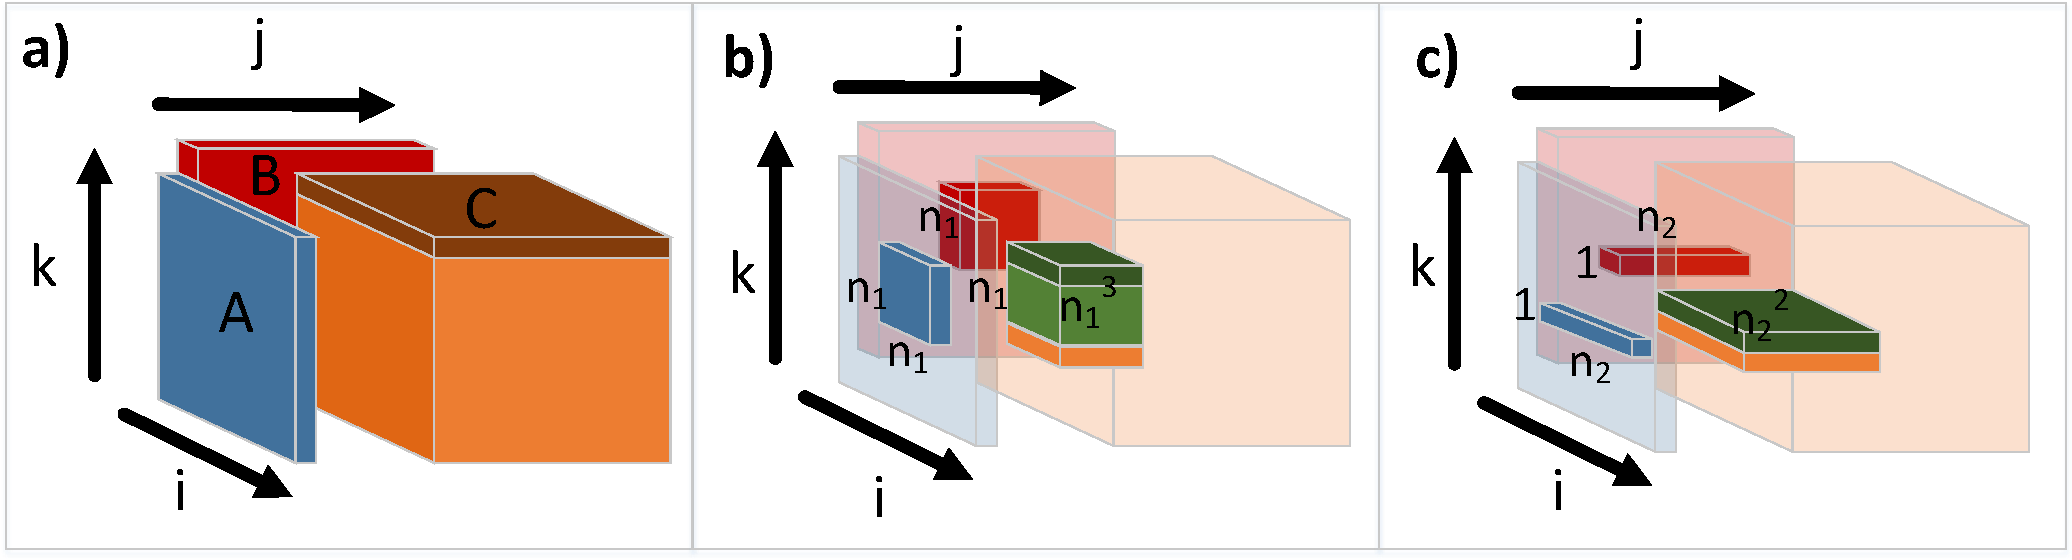
\includegraphics[width=\columnwidth]{figures/mmm_reuse}
 	\caption{Matrix-matrix multiplication subset shape problem. a) 
 		geometric interpretation of $C = A \times B$ (orange cube represents 
 		3-dimensional iteration space of partial sums, matrix C is formed by 
 		reduction over dimension $k$ - represented by dark orange plane). b) 
 		optimal surface to volume subset shape. Note that in a subsequent 
 		subset computation only one of the three planes (blue, red or dark 
 		green) can be reused. c) one of three optimal subset shapes when 
 		data reuse is considered.}
 	\label{fig:mmmreuse}
 \end{figure}

The explicit notion of reuse effects not only sequential execution, as 
discussed above, but also parallel scheduling. The number of dependency-free 
subsets in the optimal S-partition determines maximum degree of parallelism up 
to which optimal computational efficiency is maintained. Above this threshold, 
further parallelization is performed either by parallelizing dependent subsets, 
causing additional communication between processes, or by shrinking the size of 
subsets.
 Due to size constraints, the thorough analysis of different parallelization 
 schemes is presented in the Appendix.  Here we show only a comparison of 
 execution time (assuming that each I/O operation takes unit time and every 
 other operation is performed instantaneously) and parallel efficiency of three 
 schemes (Table \ref{tab:mmmEfficiency} and Figure \ref{fig:mmmScaling}): 
\begin{enumerate}
	\item \textbf{par. in IJ dim:} 
%	Subset 
%	size is determined by Equation 
%	\ref{eq:flat}. 
%	The reduction among the \textbf{k} 
%	dimension is performed by a single process. Above the maximum degree of 
%	parallelism threshold the 
%	subsets' size is reduced.
	Parallelization is done only on the IJ plane and the local domain size is 
	$[a \times a \times K]$, where $a = \sqrt{\frac{MN}{P}}$.
	\item \textbf{par. in ijk dim:} The subset's size is 
	constant determined by 
	Equation \ref{eq:flat} and the reduction among the \textbf{k} dimension is 
	parallelized.
	\item \textbf{cubic} 
	the local domain size is 
	$[a_c \times a_c \times a_c]$, where $a_c = 
	\min\{\big(\frac{MNK}{P}\big)^{1/3}, 
	\sqrt{\frac{S}{3}}\}$ (Equation \ref{eq:cubic}).
%	The subset's size is constant 
%	determined by Equation 
%	\ref{eq:cubic}, above the threshold 
%	the reduction among the \textbf{k} dimension is parallelized.
\end{enumerate}

Knowing the analytical solution for those three schemes, our S-partition 
algorithm chooses the optimal one for given set of parameters. 


\textbf{Notes:}

\begin{itemize}
	\item If $M = N$, then \textbf{par. in ij dim} scheme reduces to 2D 
	decomposition (e.g., Cannon's algorithm). 
	\item If $M = N = K$ then \textbf{par. in ijk dim} scheme reduces to 2.5D 
	decomposition.
	\item CARMA asymptotically reaches \textbf{cubic} scheme, guaranteeing that 
	the longest dimension of local cuboid is at most two times larger than the 
	smallest one.
\end{itemize}



\begin{table*}[t]
\begin{tabular}{lllll}
\toprule
range & metric & par in \textbf{ij} dim & par. in \textbf{ijk} dim & cubic \\
\midrule 
%		& $t(p,S)$ & $E(p,S)$ & $t(p,S)$ & $E(p,S)$ & $t(p,S)$ & $E(p,S)$ \\
\multirow{2}{*}{$p \le \frac{nm}{S}$} & $t(p,S)$ & $\frac{2nmk}{p\sqrt{S}}$ & $\frac{2nmk}{p\sqrt{S}}$ & $\frac{2\sqrt{3}nmk}{p\sqrt{S}}$ \\
& $E(p,S)$ & 1 & 1 & 	$\frac{1}{\sqrt{3}}$\\
\midrule 
\multirow{2}{*}{$\frac{nm}{S} < p \le \frac{3nm}{S}$} & $t(p,S)$ & $2k 
\sqrt{\frac{nm}{p}}$ & 
$\frac{2nmk}{p\sqrt{S}} + S$ & $\frac{2\sqrt{3}nmk}{p\sqrt{S}}$ 
\\
& $E(p,S)$ & $\sqrt{\frac{nm}{pS}}$ & $\frac{1}{1 + 
\frac{pS^{3/2}}{2nmk}}$ & 	$\frac{1}{\sqrt{3}}$ \\
\midrule \\
\multirow{2}{*}{$\frac{3nm}{S} < p$} & $t(p,S)$ & $2k 
\sqrt{\frac{nm}{p}}$ & 
$\frac{2nmk}{p\sqrt{S}} + S$ & $\frac{2\sqrt{3}nmk}{p\sqrt{S}} + 
\frac{S}{3}$\\
& $E(p,S)$ & $\sqrt{\frac{nm}{pS}}$ & $\frac{1}{1 + 
\frac{pS^{3/2}}{2nmk}}$ &	$\frac{1}{\sqrt{3} + 
\frac{pS^{3/2}}{6nmk}}$
\end{tabular}
\caption{Running time and parallel efficiency of the Matrix-Matrix 
multiplication for different partition schemes. Three ranges correspond 
to thresholds above which parallelization in \textbf{k} dimension is 
performed.}
\label{tab:mmmEfficiency}
\end{table*}


 \begin{figure*}[t]
 	\hspace*{-1.5cm}
 	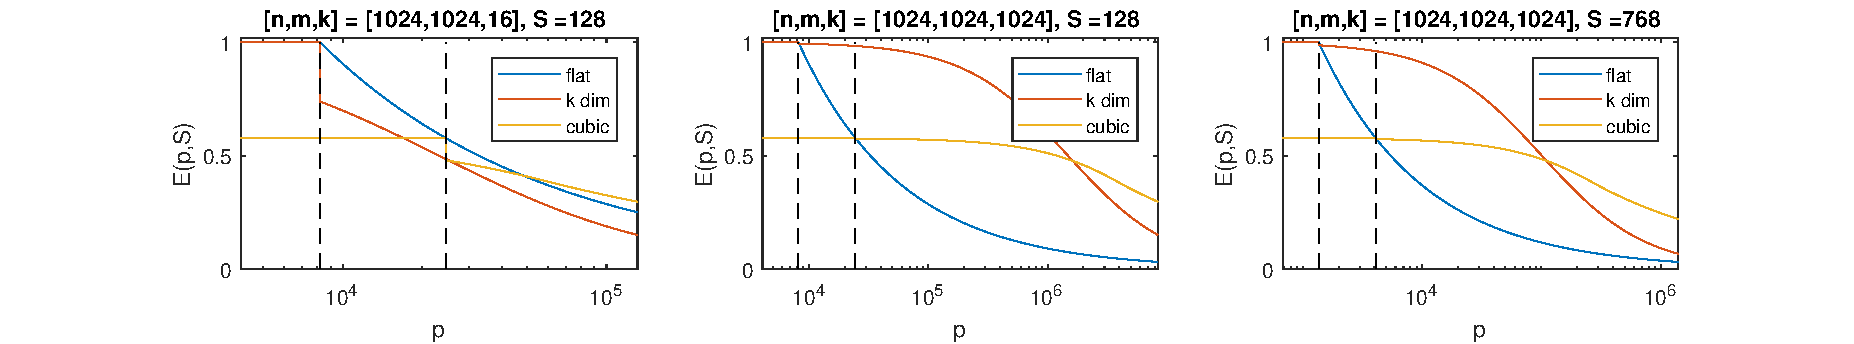
\includegraphics[width=2.5\columnwidth]{figures/mmmScaling}
 	\label{fig:mmmScaling}
 	\caption{Parallel efficiency of different partition schemes for matrix 
 		matrix multiplication. Two vertical dashed lines correspond to 
 		thresholds 
 		$nm/S$ and $3nm/S$ (Table \ref{tab:mmmEfficiency}).}
 \end{figure*}

\section{CARMA 2.0 ?}
\label{sec:implementation}
 \greg{Computation and communication overlap. will add this once we have it.}
\subsection{Recursive vs single step}
\begin{enumerate}
	\item \greg{Recursive steps determine data layout.}
	\item \greg{Manual reduction tree vs MPI collectives. Conclusion: We 
	implemented both, but on Piz daint recursive is faster, possibly due to 
	static knowledge about spatial data locality}
\end{enumerate}
\subsection{Local buffer reuse}
\greg{We use two buffers instead of $\log P$}
\subsection{Block recursive data layout}
\begin{enumerate}
	\item \greg{Faster, doesn't require reshuffling in each step}
	\item \greg{Better suitable for integration with ScaLAPACK ?}
\end{enumerate}


\section{Evaluation}
\label{sec:evaluation}

\subsection{Test cases}
\greg{Describe where do the skinny matrices show up, why they are important, 
why strong scaling (even suboptimal) is important.}
\subsection{Environment}
\greg{Piz daint description}
\subsection{Results}
\greg{I believe the scenarios should cover, both weak and strong scaling (I 
don't know in which order):
\begin{itemize}
	\item "Standard" square scenario. Marko - we are still the fastest even for 
	square case?
	\item "CARMA" scenarios. Power of 2, one and two "large dimensions"
	\item "Our case" scenarios. Non power of 2, rectangular matrices. Is it 
	fair to assume that original CARMA pads matrices with zeros to match the 
	closest power of 2?
\end{itemize}
Should we add intra node evaluation too? Or do we care only about the 
distributed case?
}


%\begin{multline}
%\\
%G = (V,E) \\
%|V| = n \\
%|E| = m \\
%p partitions \\
%\forall_{i = 1..p} P_i \in V \\
%\bigcup_{i = 1..p} P_i = V \\
%\bigcap_{i = 1..p} P_i = \emptyset \\
%\forall_{i = 1..p} BE_i \in E = \{(u,v) : u \in P_i \land v \notin P_i\} \\
%\forall_{i = 1..p} BV_i \in V = \{u : (u,v) \in BE_i\} \\
%pl_i(u,v) = \{e \in E \cap (P_i \times P_i) : \text{edges connect u and v} \} 
%- 
%\text{local path between u and v} \\
%pr_i(u,v) = \{e \notin E \cap (P_i \times P_i) : \text{edges connect u and v} 
%\} - \text{remote path between u and v} \\
%\end{multline}
%\begin{enumerate}
%	\item For each $P_i$:
%\end{enumerate}

\section{Related work}
\begin{enumerate}
	\item \greg{I/O minimization in general, starting from pebble games, to 
	communication minimization in linear algebra.}
	\item \greg{Asymptotic complexity and the importance of constants.}
	\item \greg{Matrix multiplication algorithms.}
\end{enumerate}


%	To the best of our knowledge, in the literature there is a disparity 
%	between the work-centric and communication-centric scheduling. The former 
%	one focuses on minimizing the execution critical path by reordering and 
%	splitting tasks among the processing units (\cite{schedulingNP}). Many 
%	related scheduling problems are formulated as knapsack 
%	\cite{knapsackSched}, 
%	\cite{knapsackQuadSched} or partially ordered 
%	knapsack \cite{POKSched} optimization. Communication-centric (or 
%	communication-avoiding) approach tries to minimize the number and volume of 
%	messages exchanged across processes (e.g, \cite{SchedMaxFlow}). Many 
%	problem-specific methods are 
%	known, e.g. in linear algebra \cite{mmmSched}, \cite{communicationOptMMM}, 
%	\cite{Cholesky}, PDE solvers \cite{MeshPart} or 
%	stencil computations \cite{modesto}. For 
%	general DAG scheduling, however, the focus is mostly on different variants 
%	of balanced min-cuts of graphs \cite{balancedGraphPart}, 
%	\cite{dagPartitioningTrees}. This approach 
%	indeed lowers the 
%	communication overhead while trying to distribute work evenly. Even though 
%	balanced graph partition is also known to be NP-hard 
%	\cite{schedHardness}, \cite{partitioningHardness}, much work 
%	has been done to improve the efficiency of approximation algorithms 
%	\cite{approximatingCuts}, \cite{balancedGraphPart}.
%	
%	I/O minimizing scheduling focuses on maximizing data reuse - both spatial 
%	and temporal. Spatial data reuse orbits around vectorization and alignment 
%	techniques. Temporal reuse requires instruction reordering, like loop 
%	tiling or loop fusion. Those techniques are widely used in stencil 
%	computations (\cite{modesto}) and linear algebra 
%	(\cite{comm-avoiding-triang}). Abstractions like polyhedral model 
%	(\cite{polyhedralModel}) 
%	give powerful 
%	mathematical tools to e.g., minimize reuse distance, but they are 
%	limited to only particular class of programs. Elango et. al 
%	(\cite{redbluewhite}) worked on general class represented by CDAG, but the 
%	authors 
%	focused on I/O lower bound, without assessing its tightness or generating 
%	schedules.
%	In this work, we try to combine those two approaches. In the work-centric 
%	view, a computation DAG is viewed in a context of dependencies between the 
%	tasks and a goal is to minimize the depth - therefore, partitions tend to 
%	be aligned with a critical path. In the communication centric view, a cut 
%	size is minimized, which can result in partitions perpendicular to a 
%	critical path - loosing the grasp on the overall execution time.

\section{Conclusions}

%\section{Notes}
%NP-hardness, approximation algorithms. Is S-partition submodular ? If so, 
%look at "Fast Greedy Algorithms in MapReduce and Streaming".
%

%	\section{Bibliography}

%% Bibliography style
%\bibliographystyle{ACM-Reference-Format}
\bibliographystyle{ACM-Reference-Format}
\bibliography{mmm-ppopp}


\appendix
\section{Parallel scheduling}
\todo{Move the whole thing to appendix? Or discard it?}
In this section, we start with the reuse analysis from Section 
\ref{sec:partitionShape} 
to derive the execution time and parallel efficiency metric of the two tiling 
schemes of Matrix-Matrix multiplication. In this framework, we assume that each 
I/O operation takes unit time and any arithmetic operation is performed 
instantaneously, therefore $t = Q$. We start with two observations:

\begin{enumerate}
\item There is only one dimension on 
which a reuse set projection is not empty $\exists!_{\mathbf{d}}: 
\phi_{\mathbf{d}}(R) \ne 
\emptyset$, which implies, that there is no reuse along the plane 
perpendicular 
to this dimension. Furthermore, if $\mathbf{d} = \mathbf{k}$, meaning that 
$\mathbf{m} \times \mathbf{n} \parallel \mathbf{k}$, then if the 
parallelization is performed only on the \textbf{mn} plane, then there are 
no RAW 
conflicts discussed in Section \ref{sec:partitionShape} - subsets on 
this 
plane are embarrassingly parallel. 
\item To achieve maximum reuse (and therefore optimum usage 
of the fast memory), the subset shape must be fixed to the one derived 
in 
Section \ref{sec:partitionShape}. This means, that there is maximum 
available 
parallelism (dictated by the number of optimal subsets in one 
\textbf{mn} plane) up to which the parallel efficiency will remain 
constant. Above this threshold, we have three options: 1) reduce the 
subset size, reducing the effective memory size, 2) parallelize in 
\textbf{k} dimension, creating RAW writes and requiring additional 
communication between processes, 3) create cubic subsets, effectively 
combining 1 and 2.
\end{enumerate}

From this, we derive following formulas:

\begin{multline}
\\
a_0 = \sqrt{S+1} - 1  \text{ (size of a side of the square subset )}\\
N = \frac{nm}{a^2} \approx \frac{nm}{S} \text{ (number of optimal square 
	subsets in one \textbf{mn} plane)}\\
D_0(p,S) = |\{P \in \mathcal{P} : \forall_{P_i, P_j} \phi_{\mathbf{k}}(P_i) = 
\phi_{\mathbf{k}}(P_j)\}| = k \\
\text{number of subsets which projection along the \textbf{k} dimension is 
	equal} \\ 
\text{- because the subsets are flat, the "height" of the 
	subset stack}
\\ 
\text{in \textbf{k} dimension is k }\\
\end{multline}

Now, for the case where we do not exceed the parallelism threshold $p \le N$ : 
\begin{multline}
\\
t_0(p,S) = \frac{N}{p} (\mathcal{S}_0 - r_0) D_0(p,S) = \frac{2nmk(\sqrt{S+1} 
	- 
	1)}{(\sqrt{S+1} - 1)^2 p} \approx \frac{2nmk}{\sqrt{S} p} \\
E_0(p,S) = \frac{t_0(1,S)}{p t_0(p,S)} = 1 \\
\end{multline}

If $p > N$, we have two previously discussed cases: smaller square tiles and 
parallelization in \textbf{k} dimension. Case 1:
\begin{multline}
\\
D_1(p,S) = D_0(p,S) \\
a_1 = \sqrt{\frac{nm}{p}} \text{ size of a side of the reduced square 
	subset} \\
\mathcal{S}_1 - r_1 = 2a_1 = 2\sqrt{\frac{nm}{p}} \text{ number of load 
	operations per one subset} \\
t_1(p,S) = (\mathcal{S}_1 - r_1) D_1(p,S) = 2k \sqrt{\frac{nm}{p}} \\
E_1(p,S) = \frac{t_0(1,S)}{p t_1(p,S)} = \sqrt{\frac{nm}{Sp}} \\
\end{multline}

Case 2 (parallelization in \textbf{k} dimension): 

\begin{multline}
\\
D_2(p,S) = \frac{D_0(p,S)N}{p} \text{ (the depth is reduced by } \frac{N}{p} 
\text{)}\\
a_2 = a , \mathcal{S}_2 = \mathcal{S}_0\\ 
r_2 = a_2^2(1 - \frac{p}{Nk}) \text{ (in every $\frac{p}{N}$ plane in dimension 
	\textbf{k} we} \\
\text{communicate whole $a_2^2$ plane between subsets)} \\
t_2(p,S) = (\mathcal{S}_2 - r_2) D_2(p,S) = \frac{2nmk}{\sqrt{S}p} + S \\
E_2(p,S) = \frac{t_0(1,S)}{p t_2(p,S)} = \frac{1}{1 + \frac{\sqrt{S}p}{2nmk}} \\
\end{multline}

Case 3 (cubic subsets - Section \ref{sec:subsetShape}):

\begin{multline}
\\
a_3 = \sqrt{\frac{S}{3}} \\ 
\mathcal{S}_3 = 3a_3^2, r_3 = a_3^2\\ 
D_3(p,S) = \frac{nmk}{p \Big(\frac{S}{3}\Big)^{\frac{3}{2}}}\\
\\
\frac{nm}{S} \le p < \frac{3nm}{S} :\\
t_3(p,S) = (\mathcal{S}_3 - r_3) D_3(p,S) = \frac{2\sqrt{3}mnk}{\sqrt{S}p} \\
E_3(p,S) = \frac{t_1(1,S)}{p t_3(p,S)} = \frac{1}{\sqrt{3}}\\
\\
p > \frac{3nm}{S} :\\
t_3(p,S) = (\mathcal{S}_3 - r_3) D_3(p,S) = \frac{2\sqrt{3}mnk}{\sqrt{S}p} \\
E_3(p,S) = \frac{t_1(1,S)}{p t_3(p,S)} = \\
\end{multline}

$$2 \cdot h_{Sopt}(G) \ge \sum_{P \in \mathcal{P}(G)} h_{Sopt}(inv(P)) $$
$$ \nexists_{P \in \mathcal{P}}: V_{w,opt} \in P $$

%\begin{algorithm}
%	\label{alg:spartition}
%	\SetKwInOut{Input}{Input}
%	\SetKwInOut{Output}{Output}
%	\underline{rSpartitionCut}\;

\end{document}
